
\documentclass[conference,a4paper]{IEEEtran}
\IEEEoverridecommandlockouts
% The preceding line is only needed to identify funding in the first footnote. If that is unneeded, please comment it out.
\usepackage{amsmath,amssymb,amsfonts,dsfont,bm}
\usepackage{algorithmic}
\usepackage{graphicx}
\usepackage{booktabs, tabularx}
\usepackage{subcaption}
\usepackage{textcomp}
\usepackage{xcolor}
\usepackage{enumitem}
\usepackage{parskip}
\usepackage{natbib}
%\usepackage[top=1cm,left=1cm,right=1cm,bottom=2cm]{geometry}
\bibliographystyle{plainnatnourl}
\usepackage{hyperref}
\usepackage{cleveref}


\textheight 26cm

\begin{document}

\renewcommand*{\ttdefault}{cmvtt}

%\title{Cooperative Multi-agent Reinforcement Learning for Conveyor Belt Pick-and-Place Robots\\
\title{Factory Manipulation with Cooperative\\ Multi-agent Reinforcement Learning\\
{\footnotesize }
% \thanks{Identify applicable funding agency here. If none, delete this.}
}

\author{\IEEEauthorblockN{Nikolas Kirschstein}
\IEEEauthorblockA{\textit{Student no.  03782928} \\
\textit{Technical University of Munich}\\
{\url{nikolas.kirschstein@tum.de}}}
\and
\IEEEauthorblockN{Kassian Köck}
\IEEEauthorblockA{\textit{Student no. 03779568} \\
\textit{Technical University of Munich}\\
\url{kassian.koeck@tum.de}}
}

\maketitle

\begin{abstract}
Efficient factory automation is crucial for modern manufacturing, but traditional pre-programmed approaches often fall short in handling dynamic and complex tasks. This report investigates the application of cooperative multi-agent reinforcement learning to address these challenges in a simulated factory environment. By training multiple robot arms to collaborate in transporting and sorting objects, we aim to optimise efficiency and adaptability in factory manipulation. Our results show that training successfully cooperating agents is hard and time-consuming as well and can, up to now, only be achieved for a simplified problem setting.
\end{abstract}

\vspace{1em}
\def\IEEEkeywordsname{Keywords}

\begin{IEEEkeywords} \itshape
multi-agent reinforcement learning;
cooperation;
multi-robot coordination;
industrial robotics;
factory manipulation;
pick-and-place tasks;
moving conveyor belt.
\end{IEEEkeywords}





\section{Introduction}

\subsection{Motivation}

In today's industrial and logistics environments, factory manipulation tasks such as automated pick-and-place (P\&P) play a key role. 
Our work addresses a critical challenge: optimising the performance of robotic co-manipulation in a factory, leading to improvement in efficiency and reduced costs.
We utilise multi-agent reinforcement learning (RL) to control the movements of robot arms in a factory setting. 
This method offers significant advantages over traditional control techniques.
Conventional robotic picking systems \citep[cp.][]{carbonell_coordinated_1998,bozma_multirobot_2012,yu_multi-robot_2017,han_toward_2020} rely on pre-programmed motions, requiring precise planning for every possible item configuration, particularly in scenarios involving multiple robots with overlapping workspaces. 
Those approaches are time-consuming, inflexible, and expensive to maintain.
In contrast, multi-agent RL allows to learn near-optimal cooperative behaviour simply from environmental interactions in an end-to-end fashion.
We adopt a multi-agent learning approach for factory manipulation problems in the representative and common setting of P\&P along a moving conveyor belt. Our open-source implementation is available at \url{https://github.com/nkirschi/tum-adlr-007}.

\subsection{Related Work}

Exploring the optimisation of robotic co-manipulation on conveyor systems through multi-agent RL remains a mostly unexplored domain, particularly concerning real-world complexities.
In the only line of work we are aware of, \citet{lan_towards_2021,lan_coordination_2022} employ deep Q-learning  to obtain a global puppeteer policy, but not true multi-agent RL with partially observable state space. To tackle partial observability, there exists a myriad of methods and paradigms in the multi-agent literature \citep{nguyen_deep_2020}. A much-noticed study conducted by \citet{peng_facmac_2021} introduces FACMAC, a cooperative multi-agent RL algorithm well-suited for managing factored critic structures. 
To enhance the system, \citet{muglich_equivariant_2022} integrate equivariant networks that are able to leverage symmetry in the environment, which is usually present in the factory context.
This integrated approach holds promise for significantly improving collaboration and efficiency in robotic P\&P endeavours.

\subsection{Report Structure}
\Cref{sec:setup} describes our technical setup in detail, \Cref{sec:shaping} explains the reward shaping process, \Cref{sec:continuous,sec:discrete} discuss our results for a continuous and a discrete notion of control, respectively, and \Cref{sec:conclusion} concludes the report.


\section{Our Setup}
\label{sec:setup}


\subsection{The Environment}

For lack of a real-world factory environment, our work considers a simulated environment created by \citet{rostel_factory_2024} based on DeepMind's MuJoCo physics engine \citep{howell_predictive_2022}. As shown in \Cref{fig:env}, it consists of an accelerating conveyor belt transporting cuboid objects, and an even number of robot arms along both sides of the conveyor belt. The spawn frequency of new cubes linearly increases with the number of arms. The robots are tasked with picking cubes from the belt and placing them in their side's basket, one at a time. The per-bucket score is incremented by one whenever a new cube is successfully placed. Once a cube is missed by all robots, or an arm collides with anything, the episode ends. The objective is maximising the sum of the bucket scores, i.e., the total number of cubes collected within an episode.

\begin{figure}[t]
	\centering
	\begin{subfigure}[b]{0.45\linewidth}
		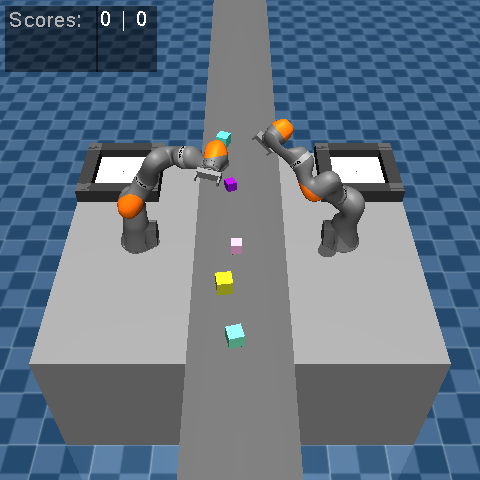
\includegraphics[width=\linewidth]{figures/screenshot_two_arms.png}
		\caption{two arms}
		\label{fig:two-arms}
	\end{subfigure}
	\hfill
	\begin{subfigure}[b]{0.45\linewidth}
		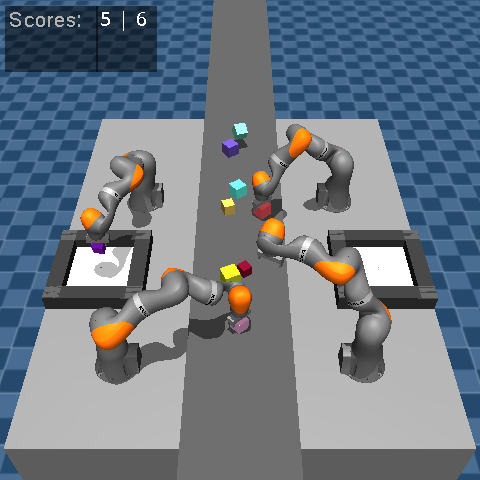
\includegraphics[width=\textwidth]{figures/screenshot_four_arms.png}
		\caption{four arms}
		\label{fig:four-arms}
	\end{subfigure}
    
	\caption{The MuJoCo-based factory simulation considered in this work. Note that the displayed score indicator is per bucket rather than per arm.}
	\label{fig:env}
\end{figure}



\subsection{The IK Base Policy}

As a pre-programmed baseline to compare our RL agents to, we employ a classic inverse kinematics (IK) policy.
It operates as a state machine\footnote{Seven states: \texttt{IDLE}, \texttt{GO\_TO\_GRASP}, \texttt{GRASP\_APPROACH}, \texttt{GRASP\_CLOSE}, \texttt{POST\_GRASP}, \texttt{GO\_TO\_RELEASE}, \texttt{RELEASE}}, sequentially handling individual target objects within the environment. 
Joint angles for control are calculated via IK based on the desired position of the current target object.
Each instance of the policy functions independently, disregarding the positions of other arms but considering the target objects of other instances. 
While effective in single-arm scenarios, this approach suffers from a high collision rate when multiple arms are involved, hindering its applicability in complex, multi-agent environments.

\subsection{The Control}

To investigate the effectiveness of RL in this context, we employ two classes of control scenarios, which are summarised in \Cref{tab:control-definitions}.
In the full joint control scenario, the goal is to directly learn policies for controlling the robot arms in all their degrees of freedom using RL. 
In the IK toggling scenario, RL acts as a higher-level coordinator for IK base policy-controlled arms. 
By comparing these approaches, we aim to assess the benefits and limitations of each method in addressing the complex challenges of cooperative factory manipulation.


\begin{table}[t]
\centering
\caption{Overview of control definitions, where \(n\) refers to the number of arms, \(\mathtt{DOF}\) their degrees of freedom for moving and grasping, \(N\) is the maximum number of simultaneously present objects, and \(d\) the number of parameters needed to describe an object's pose and velocity. Throughout this work, \(n \in \{2, 4\}\), \(\;\mathtt{DOF} = 7 + 1\), \(\;N = 10\), \(\;\)and \(\;d = 7 + 6\).}
\begin{tabularx}{\linewidth}{p{1.6cm}XX}
\toprule
 & 
full joint control\newline  (\Cref{sec:continuous}) & 
IK toggling control\newline (\Cref{sec:discrete}) \\\midrule

\textbf{action space} &
\([-1,1]\) \newline per joint and arm &
\(\{\textsc{on}, \textsc{off}\}\) \newline per arm \\\midrule

\bfseries observation \newline space &
\(\mathbb{R}^{n \cdot \mathtt{DOF} + N \cdot d}\) \newline
joint and cube states
&
\(\mathbb{R}^{n \cdot \mathtt{DOF} + N \cdot d + n \cdot \mathtt{DOF}}\) \newline
joint and cube states \newline {+ proposed IK control}
\\\midrule
\bfseries experimental \newline choices &
learning scope \newline ({\itshape from-scratch, delta, base})
&
\textsc{off} behaviour  \newline ({\itshape pause, retreat, base})
\\\bottomrule
\end{tabularx}
\label{tab:control-definitions}
\end{table}



\subsection{The Training}

We train all RL agents using the Stable Baselines 3 implementation \citep{raffin_stable-baselines3_2021} of the state-of-the-art on-policy Proximal Policy Optimisation (PPO) algorithm with a discount factor of 0.99 for a maximum number of five million time steps. The policy network is an MLP with two hidden layers containing 128 neurons each.


\section{Reward Shaping}
\label{sec:shaping}

\subsection{Additional Incentives}

Due to the discrete, highly sparse reward, if only the score of the buckets is used, with simply performing random movements, a positive reward is extremely unlikely, making it difficult to train with this reward.
For this reason, a denser reward function is required.
We define two incentives in addition to the score:

\begin{center}
\begin{tabular}{r l}
$I_0$: & \itshape Reward new cubes placed into bucket\\
$I_1$: & \itshape Reward the gripper approaching the closest cube\\
$I_2$: & \itshape Reward the closest cube approaching the bucket
\end{tabular}
\end{center}
Incentives $I_1$ and $I_2$ also penalise retreat from the target with negative rewards, preventing the arms from learning to oscillate for better accumulated rewards. 
The overall reward function is now a weighted average of these incentives plus a constant offset \(r_0\):
\[r = r_0 + \omega_0I_0 + \omega_1I_1 + \omega_2I_2\]
The base reward \(r_0\) is needed to "keep the episode running". Without it, particularly at the beginning of an episode when the cubes are moving on the conveyor belt and part of it away from the bucket, the average reward would be negative. As a result, the RL agent would learn to terminate the episode (e.g., by hitting the environment) to avoid accumulating negative reward.

When an arm scores, the cube is removed, and thus the distance to the closest cube as well as the distance of this cube to the bucket suddenly skyrocket in this time step. 
To avoid an outlier negative reward signal, $I_1$ and $I_2$ should be ignored for this single time step, resulting in
\begin{align*}
r &= r_0 + \begin{cases}
    \omega_0 I_0, & \text{if } I_0 > 0 \\
    \omega_1 I_1 + \omega_2 I_2, & \text{otherwise.}
\end{cases}
\end{align*}

\subsection{Parameter Choice}

The rewards for the intermediate goals of approaching the cube and bringing the cube to the bucket are necessary to obtain a less sparse reward function. However, their reward should not override the reward of the ultimate goal: the score. It has been found that, for this reason, $\omega_0$ should be at least twice as high as $\omega_1$ and $\omega_2$.

When an arm has a cube in its gripper and is positioned directly above the bucket, the incentives $I_1$ and $I_2$ are opposed. 
To avoid getting stuck in a local minimum that can occur for $\omega_1 > \omega_2$, it is best to set \(\omega_2\)  strictly larger than \(\omega_1\). Our investigations suggest a ratio \(\frac{\omega_2}{\omega_1}\) between \(1.5\) and \(2\).

If the base reward is too low, even the IK base policy has parts of the episode where the reward is negative. For instance, when the gripper is lifting the cube from the conveyor belt (which the base policy performs vertically), the distance to the bucket (located at height 0) increases. The reward should be large enough to handle these fluctuations. On the other hand, if the base reward is too high, it overpowers the other incentives. This hinders the learning process and makes the RL agent learn only to keep the episode running. Our investigations suggest choosing \(r_0\) between $2\omega_1$ and $0.5\omega_0$.

Overall, we have the following constraints:
\begin{align*}
2\omega_1 < r_0 < 0.5 \omega_0 \\
1.5 \omega_1 < \omega_2 < 2\omega_1
\end{align*}
Note that \(w_0 \ge 2w_1, 2w_2\) is implied by the other two constraints. Furthermore, the parameters can be scaled by a constant without affecting the learning process, so w.l.o.g. we can fix \(\omega_0 = 1\). Our final experiments use the following values:
\begin{align*}
r_0 = 0.4, \;\omega_0 = 1, \;\omega_1= 0.2,  \;\omega_2 = 0.4
\end{align*}
With these, a typical reward evolution of the IK base policy looks as shown in \Cref{fig:reward-timeline}.
There, the four big spikes indicate a score increment. The large negative spikes around the time steps 45, 140, 180, and 270 correspond to an arm attempting to grab a cube and lifting it.


\begin{figure}
  \centering
  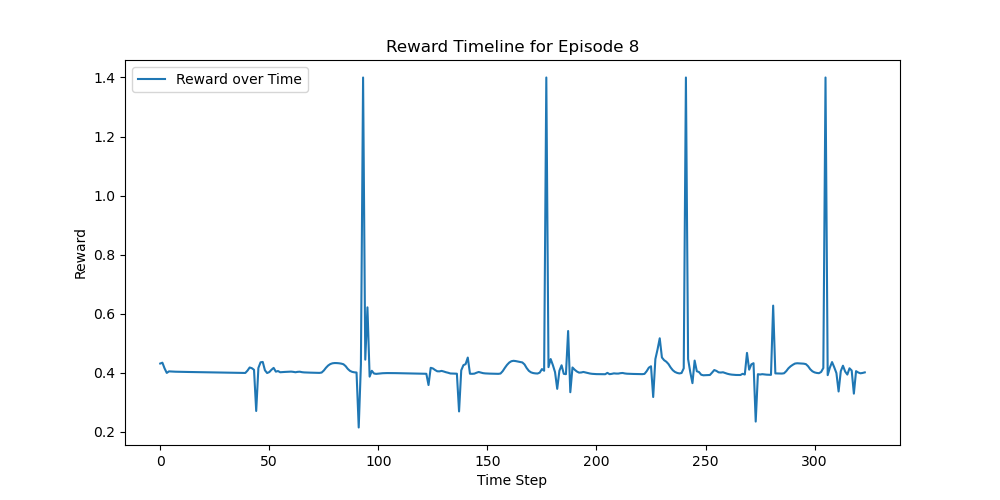
\includegraphics[width=0.5\textwidth]{figures/reward_timeline.png}
    \caption{The reward function over time in typical episode of the IK base policy with a single arm acting.}
  \label{fig:reward-timeline}
\end{figure}


\section{Full Joint Control}

\label{sec:continuous}

\subsection{Setting}

In the continuous control setting, the RL agents directly learn policies for controlling robot arm joint states. 
Each joint's action is represented by a scalar in \([-1,1]\), enabling precise control. The agent observes the robot's joint states and the positions of the cubes in the environment. 
We explore two learning approaches: learning the entire joint control policy from scratch, and delta learning, where the agent learns an optimal deviation from the IK base policy. 
To establish a baseline, we also execute the IK base policy without any learning.


\subsection{Results}

Even in the simplest case of \(n = 2\) robots, using the true sparse reward (\( \omega_0 = 1\), \(r_0, \omega_1, \omega_2 = 0\)) yields no discernible learning, resulting in essentially random agent behaviour. 
To encourage more utilisation of the IK base policy in the delta case, we initially considered an additional penalty term based on the magnitude of the deviation, which, however, did not lead to any improvement.
Incorporating a progress-based reward, as outlined in \Cref{sec:shaping}, affords a slight improvement, with the agents successfully learning to avoid collisions and attempting, but not succeeding at, grasps. 
As shown in \Cref{tab:results-continuous}, the average episode duration increases compared to the base reward condition. 
Additionally, the primary cause of episode termination shifts from collisions to missed cubes, a contrast to the base execution, where collisions are the predominant termination factor. 
However, neither the from-scratch nor the delta learnt agents exhibit any instances of successful gripping, indicating a significant challenge in mastering this complex task.



\section{IK Toggling Control}
\label{sec:discrete}

\subsection{Setting}

Due to the immense challenges posed by the continuous control setting, we introduce the IK toggling control setting as a simplification to verify that learning successful cooperation is possible at all. 
While the arms still rely on the IK base policy for low-level control, a higher-level coordinator agent determines when to activate or deactivate individual arms. 
This leads to a heavily reduced action space for each robot arm, which is now binary.
The coordinator's observation space includes the joint and cube states like before, as well as the proposed actions from the IK base policy. 
When activated by the coordinator, an arm executes its base policy. 
Upon deactivation, there are two fundamental strategies: either the arm maintains its current position until reactivated (\emph{pause}), or it returns to a predefined safe position (\emph{retreat}). 
As a baseline, we again employ the pure IK base policies without any learning from the coordinator (\emph{base}).


\subsection{Results}

Contrary to the full joint control setting, the coordinator agent manages to improve upon the baseline, even in the more complex setting of \(n = 4\) arms, the results of which are shown in \Cref{tab:results-discrete}. The \emph{pause} strategy achieves higher basket scores than both the two-arm and four-arm baselines but only outperforms the four-arm baseline in episode length. The \emph{retreat} strategy also outperforms the two-arm baseline's episode length to the same extent as the \emph{from-scratch} and \emph{delta} learning approaches. However, while it has the highest single basket score out of all experiments, it fails to score any cubes at all in the other basket, which our investigations suggest results from overly cautious behaviour involving premature retreating on that side of the belt.

\begin{table}
\caption{Test results averaged over 100 episodes}
\begin{subtable}{\linewidth}
	\centering
	\caption{Full joint control on two arms}
	\begin{tabular}{lll}\toprule
	learning scope & avg episode score & avg episode length \\\midrule
	\itshape from-scratch & $(0, 0)$ & $\mathbf{219.9}$ \\\midrule
	\itshape delta & $(0,0)$ & $\mathbf{220.5}$ \\\midrule
	\itshape base & $\mathbf{(1.65, 1.17)}$ & $208.8$ \\\bottomrule
	\end{tabular}
	\label{tab:results-continuous}
\end{subtable}
\vspace{5mm}

\begin{subtable}{\linewidth}
	\centering
	\caption{IK toggling control on four arms}
	\begin{tabular}{lll}\toprule
		\textsc{off} behaviour & avg episode score & avg episode length \\\midrule
		\itshape pause & $\mathbf{(2.01, 1.5)}$ & $173.04$ \\\midrule
		\itshape retreat & $(0, 2.12)$ & $\mathbf{216.74}$ \\\midrule
		\itshape base & $(1.18, 1.16)$ & $119.74$ \\\bottomrule
	\end{tabular}
	\label{tab:results-discrete}
\end{subtable}
\end{table}
\vspace{5mm}


\section{Conclusion and Future Work}
\label{sec:conclusion}

We employed multi-agent RL to enable cooperative behaviour of robots in a factory environment. Due to the extreme sparsity of the true reward signal, we had to perform reward shaping and experiment with different control definitions. While in the continuous full control case the problem appears too hard for the RL agents to learn any kind of gripping, the simplified discrete IK toggling setting allows the robots to cooperate successfully and outperform the IK base policy even without the shaped reward. Overall, training successful agents turned out to be just as time-consuming and expensive as classical pre-programmed control techniques, making the usefulness of RL in this domain questionable.

Future work is advised to interpolate between our continuous and discrete settings to find the least restrictive control definition where the IK base policy can still be outperformed. Moreover, the introduction of auxiliary tasks (e.g., grip, carry, release) and curriculum learning may alleviate the sparsity issues and push the boundary further towards the full joint control side.  In the same vein, the recently published causality-aware actor-critic algorithm \cite{ji_ace_2024} promises to improve exploration quality during training such that successful gripping might happen by chance.

\clearpage


\bibliography{literature}

\end{document}